%%%%%%%%%%%%%%%%%%%%%%%%%%%%%%%%%%%%%%%%%%%%%%%%%%%%%%%%%%%%
\section{智能体{}AI 信任层}
\label{sec:trust-layer}

本节描述智能体{}AI 信任层（Agentic AI Trust Layer），包含认证工作流以及 \cite{rajagopalan2025prompts} 中描述的认证提示与上下文。所有九个框架通过轻量框架适配器（framework adapter）映射到信任层。信任层包含提供核心服务（身份、策略、日志、路由）的控制平面（control plane）、与企业基础设施（IAM、PKI、SIEM、存储等）的集成、验证网关（边车 PEP）以及在智能体应用中嵌入 PEP 的客户端库。受篇幅所限，我们重点讨论关键设计要素，而非详尽概述。

\begin{figure}[t]
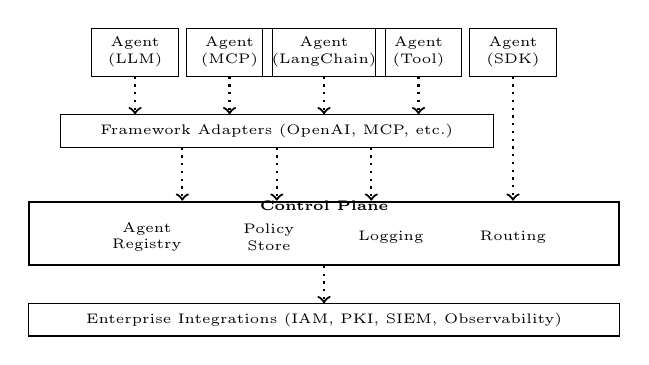
\begin{tikzpicture}[
  agent/.style={rectangle, draw, minimum width=1.1cm, minimum height=0.4cm, font=\tiny, align=center},
  integration/.style={rectangle, draw, minimum width=7.5cm, minimum height=0.4cm, font=\tiny, align=center},
  service/.style={rectangle, minimum width=1.65cm, minimum height=0.5cm, font=\tiny, align=center},
  adapter/.style={rectangle, draw, minimum width=5.5cm, minimum height=0.4cm, font=\tiny, align=center}
]

% Top layer: 5 Agents
\node[agent] (agent1) at (-2.4,0) {Agent\\(LLM)};
\node[agent] (agent2) at (-1.2,0) {Agent\\(MCP)};
\node[agent] (agent3) at (0,0) {Agent\\(LangChain)};
\node[agent] (agent4) at (1.2,0) {Agent\\(Tool)};
\node[agent] (agent5) at (2.4,0) {Agent\\(SDK)};

% Framework Adapters layer (narrower, slightly wider to accommodate 4 agents)
\node[adapter] (adapters) at (-0.6,-1) {Framework Adapters (OpenAI, MCP, etc.)};

% Control Plane box (full width, reduced height)
\node[draw, thick, rectangle, minimum width=7.5cm, minimum height=0.8cm] (controlplane-box) at (0,-2.3) {};

% Control Plane label (centered at top inside box, bold)
\node[font=\tiny\bfseries] at (0,-1.95) {Control Plane};

% Services inside control plane - single row, all same size
\node[service] (registry) at (-2.25,-2.35) {Agent\\Registry};
\node[service] (policy) at (-0.7,-2.35) {Policy\\Store};
\node[service] (logging) at (0.85,-2.35) {Logging};
\node[service] (routing) at (2.4,-2.35) {Routing};

% Bottom layer: Enterprise Integrations
\node[integration] (integrations) at (0,-3.4) {Enterprise Integrations (IAM, PKI, SIEM, Observability)};

% Arrows: First 4 agents to Framework Adapters (vertical)
\draw[->, thick, dotted] (agent1.south) -- (agent1.south |- adapters.north);
\draw[->, thick, dotted] (agent2.south) -- (agent2.south |- adapters.north);
\draw[->, thick, dotted] (agent3.south) -- (agent3.south |- adapters.north);
\draw[->, thick, dotted] (agent4.south) -- (agent4.south |- adapters.north);

% Arrows: 3 parallel vertical arrows from Framework Adapters to Control Plane
\draw[->, thick, dotted] ([xshift=-1.2cm]adapters.south) -- ([xshift=-1.2cm]adapters.south |- controlplane-box.north);
\draw[->, thick, dotted] (adapters.south) -- (adapters.south |- controlplane-box.north);
\draw[->, thick, dotted] ([xshift=1.2cm]adapters.south) -- ([xshift=1.2cm]adapters.south |- controlplane-box.north);

% Arrow: Direct SDK agent bypasses adapters to Control Plane (vertical)
\draw[->, thick, dotted] (agent5.south) -- (agent5.south |- controlplane-box.north);

% Control Plane connects to Enterprise Integrations (vertical)
\draw[->, thick, dotted] (controlplane-box.south) -- (integrations.north);

\end{tikzpicture}
\caption{智能体{}AI 信任层。}
\label{fig:runtime-architecture}
\end{figure}

\subsection{架构}

图~\ref{fig:runtime-architecture} 展示了信任层架构，其中智能体与控制平面交互。

\textbf{框架适配器（Framework Adapters）}。每个框架通过轻量适配器集成，将框架原生操作转换为认证工作流。适配器实现四阶段协议——注册、调用签名、验证和证言——同时呈现框架原生 API。集成是透明的；开发者使用标准框架 API（MCP 服务器、OpenAI 客户端、LangChain 智能体），密码学强制执行自动发生。

\textbf{控制平面服务}。控制平面提供四项核心服务：
\begin{itemize}
\item \textit{智能体注册中心（Agent Registry）}：存储智能体标识符和公钥，以及智能体内工具的标识符和公钥，保留密码学谱系。支持即时凭证撤销。PEP 在签名验证期间检索公钥。

\item \textit{策略存储（Policy Store）}：防篡改的策略存储，PEP 从中检索并通过交集组合层级策略（如公司、业务单元、团队）。

\item \textit{路由（Routing）}：跨网络边界在智能体之间路由签名调用，使被调用方能够获取调用方的公钥进行验证。

\item \textit{日志（Logging）}：通过防篡改哈希链记录所有安全事件及其密码学谱系。与企业 SIEM（安全信息与事件管理）平台集成。被阻止的操作生成结构化日志，标明拒绝原因（签名无效、策略违反、缺少证言、验证器失败），包含足够的调试细节同时避免策略泄露。审计日志支持根因分析和合规报告。
\end{itemize}

\textbf{分布式执行}。这些服务以高可用配置运行，与企业基础设施（IAM、PKI、SIEM、可观测性平台）集成。控制平面是多租户（multi-tenant）的——组织部署共享基础设施，同时保持租户间的密码学隔离。该架构实现零信任分布式验证——每个 PEP 使用注册中心的公钥和策略存储中的策略独立验证调用。PEP 默认以进程内方式嵌入（链接库）或作为边车部署，提供水平可扩展性。使用嵌入式 PEP 时，不存在集中式瓶颈；验证在每个边界本地发生，开销为亚毫秒级。管理员可以通过控制平面即时撤销凭证、更新策略或隔离智能体。受篇幅所限，完整架构细节不在本文范围内；感兴趣的读者可参阅我们的技术报告获取完整实现细节。

\subsection{设计决策}

在生产环境中实现认证工作流和信任层暴露了若干需要明确设计立场的实际挑战——我们讨论应对这些挑战的六个最有趣的设计决策。

\textbf{身份桥接（Identity Bridging）}。企业身份需要跨框架桥接——每个框架有自己的认证模型（OAuth、API 密钥、SAML）。我们不按框架逐一解决，而是在协议层进行桥接。用户认证时，信任层颁发绑定到其会话的临时密钥对（ephemeral keypair），并将密码学验证后的主体传播到所有框架。签名调用通过委托链携带用户身份；每个 PEP 从智能体注册中心独立验证原始主体。这集中了 IAM 集成——框架不需要各自对接企业身份系统；信任层一次性处理认证。当通过 OAuth 认证的 Alice 调用通过 API 密钥认证的 Claude，后者再调用通过 MCP 认证的工具时，日志显示"Alice via Claude accessed file"，保留审计轨迹。协议级桥接提供了更简单的编程模型和一致的主体传播，消除了按框架集成的复杂性。

\textbf{会话管理（Session Management）}。许多框架缺乏原生会话概念（MCP、LangChain 是无状态的），但跨轮次关联对安全至关重要。我们不修改每个框架来添加会话，而是在协议层使用上下文标识符和序列号透明跟踪。信任层维护认证上下文，无论框架是否支持——没有会话的框架获得透明的协议级跟踪；有会话的框架直接映射。多租户架构确保每个会话的密码学隔离上下文，防止跨会话污染。这使得跨多框架工作流的统一审计轨迹成为可能，无需修改各框架协议。

\textbf{可验证委托（Verifiable Delegation）}。多跳委托带来权限升级风险——被攻破的中间智能体可能声称拥有比授予的更大的权限。我们不依赖基于信任的委托，而是强制执行密码学范围收窄。签名委托令牌包含委托方身份、被委托方身份、范围约束和过期时间。信任层通过交集强制执行范围收窄：委托范围 = 委托方授予 $\cap$ 被委托方拥有，扩展了 MAPL 的代数（第~\ref{sec:policy}~节）。被攻破的智能体不能声称拥有比授予的更大的权限；下游服务通过密码学方式验证委托有效性。这在异构框架中提供了可证明的最小权限（least privilege）。

\textbf{前向保密（Forward Secrecy）}。长期 API 密钥带来操作和安全风险——密钥很少轮换，单次泄露就会危及所有会话。我们不依赖操作性的密钥轮换策略，而是在设计层面（by-design）使用临时密钥（ephemeral key）。每个会话获得唯一的临时密钥对，自动过期。密钥轮换通过会话（session）生命周期自然发生，无需基础设施修改，提供会话级前向保密。攻破一个会话的密钥不影响其他会话，在无操作开销的情况下限制了爆炸半径。

\textbf{大规模服务账号}。智能体系统在运行时动态生成实体——编排器（orchestrator）生成智能体，智能体生成工具，工作流创建子工作流。传统 IAM 的手动配置无法扩展到运行时动态。我们不依赖手动配置，而是在注册时（第~\ref{sec:authenticated-workflows}~节）以工具级粒度自动配置密码学身份——分配 (tool\_id, keypair) 并记录在智能体注册中心。无需手动配置、无需凭证分发、无 IAM 瓶颈。每个工具保持独立的密码学可问责性，最小化爆炸半径。这使得在企业规模下动态部署智能体成为可能。

\textbf{双向可问责性（Bidirectional Accountability）}。单向认证在智能体环境中造成问责缺口——调用方无法证明服务正确执行了操作；服务无法证明调用方请求了操作。我们不使用单向签名，而是使用双向签名实现相互不可否认性。调用方对请求签名；服务对结果签名。每个操作产生来自双方的密码学证明，提供合规级审计轨迹——服务不能否认操作；调用方不能否认请求。结合身份桥接和防篡改日志，这在异构认证边界中提供了完整的可问责性。
